\documentclass{article}
\usepackage{amsmath}
\usepackage{amssymb}
\usepackage[a4paper, top=25mm, bottom=25mm, left=25mm, right=25mm]{geometry}
\usepackage{pgfplots}
\usepackage{mathtools}
\usepgfplotslibrary{fillbetween}
\pgfplotsset{compat=1.18}

\begin{document}
\pagestyle{empty}
\large

\begin{center}
2014-2015 Fall \\MAT123 Makeup\\(28/01/2015)
\end{center}

\noindent 1. Sketch the graph of the function given by $f(x)=\ln\left(4-x^2\right)$.

\hfill

\noindent 2. Evaluate the limit $\displaystyle\lim_{x\to\infty}x\arctan\frac1x$.

\hfill

\noindent 3. A manufacturer needs to make a cylindrical can that will hold $1500$ liters of liquid. Determine the dimensions of the can that will minimize the amount of material used in its construction.

\hfill

\noindent 4. Compute the arc length of the graph of the given function $f(x)=\ln(\cos x)$ on the interval $(0,\pi/4]$.

\hfill

\noindent 5. Use the Shell Method and then the Washer Method to set up an integral (but do not evaluate) the volume of the solid generated by revolving the region bounded by the curve $y=\sqrt x$ and the lines $y=2-x$ and $y=0$ around

\hfill

\noindent (a) the $x$-axis, and

\hfill

\noindent (b) the $y$-axis,

\hfill

\noindent respectively.

\hfill

\noindent 6. The arc of the parabola $y=x^2$ from $(1,1)$ to $(2,4)$ is rotated about the $y$-axis. Find the area of the generated surface. 

\hfill

\noindent 7. Using the Integral Test, determine whether the series

\hfill

\noindent $\displaystyle\sum_{n=2}^{\infty}\frac1{n\ln n^2}$

\hfill

\noindent converges or diverges.

\hfill

\noindent 8. Find the interval of convergence of the power series

\hfill

\noindent $\displaystyle\sum_{n=1}^\infty(-1)^n\frac1{n10^n}(x-2)^n$.

\newpage

\begin{center}
2014-2015 Makeup (28/01/2015) Solutions\\
(Last update: 30/08/2025 00:40)
\end{center}

\noindent 1. $\ln x$ is defined for $x>0$. Therefore, $\ln\left(4-x^2\right)$ is defined on $(-2,2)$.

\hfill

\noindent Let us find the limit as $x\to\pm2$.

\begin{equation*}\lim_{x\to2}\ln\left(4-x^2\right)=\lim_{x\to-2}\ln\left(4-x^2\right)=-\infty\end{equation*}

\hfill

\noindent The vertical asymptotes occur at $x=\pm2$.

\hfill

\noindent Take the first derivative and find the critical points. Apply the chain rule.

\[y'=\frac d{dx}\ln\left(4-x^2\right)=\frac1{4-x^2}\cdot(-2x)=-\frac{2x}{4-x^2}\]

\hfill

\noindent A critical point occurs at $x=0$. At this point, the first derivative is $0$.

\hfill

\noindent Take the second derivative. Apply the quotient rule.

\[y''=\frac d{dx}\left(\frac{-2x}{4-x^2}\right)=\frac{-2\cdot(4-x^2)-(-2x)\cdot(-2x)}{\left(4-x^2\right)^2}=\frac{-8-2x^2}{\left(4-x^2\right)^2}\]

\hfill

\noindent No inflection points occur.

\hfill

\noindent Consider some values of the function. Eventually, set up a table and see what the graph looks like in certain intervals.

\begin{equation*}f(0)=\ln4\end{equation*}

\begin{center}
    \large
    \begin{tabular}{|c|cc|} 
    \hline
        $x$&$\left(-2,0\right)$&$\left(0,2\right)$\\
        \hline
        $y$&$(-\infty,\ln4)$&$(-\infty,\ln4)$\\
        \hline
        $y'$ sign&+&-\\
        \hline
        $y''$ sign&-&-\\
        \hline
    \end{tabular}
\end{center}

\hfill

\begin{center}
\begin{tikzpicture}
  \begin{axis}[
    axis lines = center,
    xlabel = $x$, ylabel = $y$,
    domain=-2:2,
    samples=200,
    ymin=-2, ymax=1.5,
    xmin=-3, xmax=3,
    restrict y to domain=--3:1.5,
    enlargelimits=true,
    axis line style={->},
    scale=1.4,
    ]
    \addplot[blue, thick] {ln(4-x^2)};
    \draw[dashed, red] (-2,-3)--(-2,-0.35);
    \draw[dashed, red] (2,-3)--(2,-0.35);

    \node at (-1.42,0.15) {\small $-\sqrt3$};
    \node at (1.42,0.15) {\small $\sqrt3$};
    \node at (-0.2,1.25) {\small $\ln4$};
  \end{axis}
\end{tikzpicture}
\end{center}

\newpage

\noindent 2. As $x\to\infty$, the expression is in the form $\infty\cdot 0$, which is an indeterminate form. Rationalize $x$.

\[\lim_{x\to\infty}x\arctan\frac1x=\lim_{x\to\infty}\frac{\displaystyle\arctan\frac1x}{\displaystyle\frac1x}\]

\hfill

\noindent The limit is in the form $\displaystyle\frac00$. L'Hôpital's rule suggests that we take the derivative of each side of the fraction if we encounter $\displaystyle\frac00$ or $\displaystyle\frac\infty\infty$ forms.

\begin{align*}\lim_{x\to\infty}\frac{\displaystyle\arctan\frac1x}{\displaystyle\frac1x}\overset{\text{L'H.}}{=}\lim_{x\to\infty}\frac{\displaystyle\frac1{1+\left(\frac1x\right)^2}\cdot\left(-\frac1{x^2}\right)}{\displaystyle-\frac1{x^2}}=\lim_{x\to\infty}\frac1{\displaystyle1+\frac1{x^2}}=\frac11=\boxed{1}\end{align*}

\hfill

\noindent 3. The manufacturer will minimize the use of material if the total surface is minimal. Let $V$ be the volume of the can. The volume of the can may then be expressed as follows.

\[V=\pi r^2h,\]

\hfill

\noindent where $r$ is the radius of the bottom and $h$ is the height of the can. The total surface area of the can is

\[S=2\pi hr+2\pi r^2\]

\hfill

\noindent Using the equalities $1\:\text{L}=1\:\text{dm}^3$ and $V=1500\:\text{L}$, rewrite $h$ in terms of $V$.

\[V=1500\:\text{L}=1500\:\text{dm}^3=\pi r^2h\implies h=\frac{1500}{\pi r^2}\]

\[S=\frac{3000}r+2\pi r^2\]

\hfill

\noindent To minimize $S$, take the first derivative and set to $0$ to find the critical points. Apply the quotient rule.

\[S'=-\frac{3000}{r^2}+4\pi r=0\implies r^3=\frac{3000}{4\pi}\implies r=\sqrt[3]{\frac{750}{\pi}}\]

\hfill

\noindent Using the formula $\displaystyle h=\frac V{\pi r^2}$, find the height.

\[h=\frac{1500}{\pi\left(\frac{750}{\pi}\right)^{2/3}}\]

\hfill

\noindent The dimensions for this can, in terms of the radius and height, are

\[\boxed{r=5\sqrt[3]{\frac{6}\pi}\:\text{dm},\quad h=10\sqrt[3]{\frac6\pi}\:\text{dm}}\]

\newpage

\noindent 4. The length of a curve defined by $y=f(x)$ whose derivative is continuous on the interval $a\leq x\leq b$ can be evaluated using the integral

\[S=\int_a^b\sqrt{1+\left(\frac{dy}{dx}\right)^2}\,dx.\]

\hfill

\noindent Find $\displaystyle\frac{dy}{dx}$.

\[\frac{dy}{dx}=\frac1{\cos x}\cdot (-\sin x)=-\tan x\]

\hfill

\noindent Set $a=0,\:b=\pi/4$ and find the length.

\begin{align*}S&=\int_0^{\pi/4}\sqrt{1+\left(\sqrt{-\tan x}\right)^2}\,dx=\int_0^{\pi/4}\sqrt{1+\tan^2x}\,dx=\int_0^{\pi/4}\sqrt{\sec^2x}\,dx\\\\&=\int_0^{\pi/4}\left|\sec x\right|\,dx=\int_0^{\pi/4}\sec x\,dx\qquad\left[\sec x>0\quad\text{for}\quad0<x\leq\pi/4\right]\\\\&=\ln\left|\sec x+\tan x\right|\bigg|_0^{\pi/4}=\ln\left|\sqrt2+1\right|-\ln1=\boxed{\ln\left(\sqrt2+1\right)}\end{align*}

\noindent

\hfill

\noindent 5.
\begin{center}
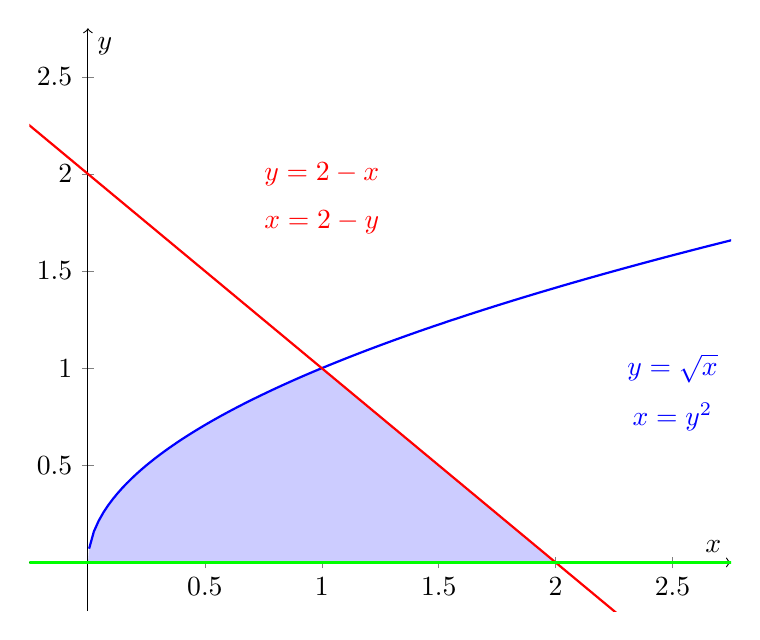
\begin{tikzpicture}
  \begin{axis}[
    axis lines = center,
    xlabel = $x$, ylabel = $y$,
    domain=-1:3,
    samples=200,
    ymin=0, ymax=2.5,
    xmin=0, xmax=2.5,
    enlargelimits=true,
    axis line style={->},
    scale=1.3,
    clip=true,
    ]
    \addplot[blue, thick, name path=A] {x^(1/2)};
    \addplot[red, thick, name path=B] {2-x};
    \addplot[green, thick, name path=C] {0};
    \addplot[blue!20, draw=none] fill between[of=B and C, soft clip={domain=1:2}];
    \addplot[blue!20, draw=none] fill between[of=A and C, soft clip={domain=0:1.01}];

    \node[red] at (1,2) {$y=2-x$};
    \node[red] at (1,1.75) {$x=2-y$};

    \node[blue] at (2.5,1) {$y=\sqrt{x}$};
    \node[blue] at (2.5,0.75) {$x=y^2$};

  \end{axis}
\end{tikzpicture}
\end{center}

\noindent (a)
\begin{align*}V_{\text{Shell}}=\int_0^12\pi y\left[(2-y)-\left(y^2\right)\right]\,dy\end{align*}
\begin{align*}V_{\text{Washer}}=\int_0^1\pi\left[\left(\sqrt x\right)^2-\left(0\right)^2\right]\,dx+\int_1^2\pi\left[\left(2-x\right)^2-\left(0\right)^2\right]\,dx\end{align*}

\hfill

\noindent (b)
\begin{align*}V_{\text{Shell}}=\int_0^12\pi x\left[\left(\sqrt x\right)-(0)\right]\,dx+\int_1^22\pi x\left[\left(2-x\right)-(0)\right]\,dx\end{align*}
\begin{align*}V_{\text{Washer}}=\int_0^1\pi\left[\left(2-y\right)^2-\left(y^2\right)^2\right]\,dy\end{align*}

\noindent 6. If the function $x=f(y)\geq0$ is continuously differentiable on $[a,b]$, the area of the surface generated by revolving the graph of $x=f(y)$ about the $y$-axis is

\[S=\int_a^b2\pi x\sqrt{1+\left(\frac{dx}{dy}\right)^2}\,dy\]

\hfill

\noindent We're interested in the right side of the parabola. So, let $f(y)=\sqrt{y}$ and set $a=1,\:b=4$. Find $\displaystyle\frac{dx}{dy}$ and then calculate the area.

\[\frac{dx}{dy}=\frac1{2\sqrt y}\]

\begin{align*}S&=\int_1^42\pi x\sqrt{1+\left(\frac1{2\sqrt y}\right)^2}\,dy=\int_1^42\pi\sqrt y\cdot\sqrt{1+\frac1{4y}}\,dy=2\pi\int_1^4\sqrt{y+\frac14}\,dy\\\\&=2\pi\left[\frac23\left(y+\frac14\right)^{3/2}\right]_1^4=\frac{4\pi}3\left[\left(\frac{17}4\right)^{3/2}-\left(\frac54\right)^{3/2}\right]=\boxed{\frac\pi6\left(17\sqrt{17}-5\sqrt5\right)}\end{align*}

\hfill

\noindent 7. Let the corresponding function be $\displaystyle f(x)=\frac1{x\ln x^2}$. $f$ is decreasing because $\ln x^2$ and $x$ are increasing for $x\geq2$. These expressions are also continuous for $x\geq2$. $f$ is positive for $x\geq2$. $x=2\implies\ln2^2=\ln4>\ln\mathrm{e}=1>0,\: x=2>0$. Since the conditions are satisfied, we may apply the Integral Test.

\hfill

\noindent Let $u=\ln x^2$, then $\displaystyle du=\frac1{x^2}\cdot 2x\,dx\implies du=\frac2x\,dx$

\[x=2\implies u=\ln2^2=\ln4,\qquad x\to\infty\implies u\to\infty\]

\begin{align*}\int_2^{\infty}\frac1{x\ln x^2}\,dx&=\int_{\ln 4}^{\infty}\frac12\cdot\frac1{u}\,du=\lim_{R\to\infty}\int_{\ln4}^R\frac{du}{2u}=\lim_{R\to\infty}\frac12\ln u\bigg|_{\ln4}^R\\\\&=\frac12\lim_{R\to\infty}\left(\ln R-\ln(\ln 4)\right)=\boxed{\infty}\end{align*}

\hfill

\noindent Since the integral diverges, the series also diverges.

\newpage

\noindent 8. Apply the Ratio Test.

\begin{align*}
\lim_{n\to\infty}\left|\frac{(-1)^{n+1}\cdot(x-2)^{n+1}}{(n+1)\cdot(10)^{n+1}}\cdot\frac{n\cdot(10)^n}{(-1)^n\cdot(x-2)^n}\right|&=\lim_{n\to\infty}\left|-\frac{n(x-2)}{10(n+1)}\right|\\\\&=\frac{|x-2|}{10}\lim_{n\to\infty}\left|\frac n{n+1}\right|=\frac{|x-2|}{10}
\end{align*}

\noindent The series converges absolutely for $\displaystyle \frac{|x-2|}{10}<1$.

\[\frac{|x-2|}{10}<1\implies|x-2|<10\implies-10<x-2<10\implies -8<x<12\]

\hfill

\noindent Investigate the convergence at the endpoints (i.e., $x=-8$ and $x=12$). Try $x=-8$.

\[x=-8\rightarrow\sum_{n=1}^{\infty}(-1)^n\frac1{n\,10^n}(-10)^n=\sum_{n=1}^{\infty}(-1)^n\cdot(-1)^n\cdot\frac1{n}=\sum_{n=1}^{\infty}(-1)^{2n}\cdot\frac1n=\sum_{n=1}^{\infty}\frac1n\]

\hfill

\noindent For $x=-8$, we get a $p$-series where $p=1$. By the $p$-series Test, it diverges. Try $x=12$.

\[x=12\rightarrow\sum_{n=1}^{\infty}(-1)^n\frac1{n\,10^n}(10)^n=\sum_{n=1}^{\infty}\frac{(-1)^n}n\]

\hfill

\noindent This is an alternating series. The non-alternating part, which is $\frac1n$, is nonincreasing for $n\geq2$ and it is positive. The limit at infinity is $0$. By Leibniz's Alternating Series Test, the series converges.

\hfill

\noindent The convergence set for the power series is

\[\boxed{\left(-8,12\right]}\]

\end{document}